\documentclass{article}
\usepackage{pgfplots}
\pgfplotsset{compat=1.13} 
\begin{document}

\begin{tikzpicture}[
    declare function={gamma(\z)=
    2.506628274631*sqrt(1/\z)+ 0.20888568*(1/\z)^(1.5)+ 0.00870357*(1/\z)^(2.5)- (174.2106599*(1/\z)^(3.5))/25920- (715.6423511*(1/\z)^(4.5))/1244160)*exp((-ln(1/\z)-1)*\z;},
    declare function={gammapdf(\x,\k,\theta) = 1/(\theta^\k)*1/(gamma(\k))*\x^(\k-1)*exp(-\x/\theta);},
    declare function={wien(\T) = 2897.8/(\T+0.01);}
]

\begin{axis}[
  no markers, domain=0:100, samples=100,
  axis lines=left, xlabel=$n_t^i$, ylabel=$f_n(.)$,
  every axis y label/.style={at=(current axis.above origin),anchor=east},
  every axis x label/.style={at=(current axis.right of origin),anchor=north},
  xtick={6.0}, ytick=\empty,
  xticklabels={$n^*$},
  enlargelimits=false, clip=false, axis on top,
  grid = major,
  xmax=10
  ]

%\addplot [very thick,cyan!20!black] {gammapdf(x,2,2)};
%\addplot [fill=cyan!20, draw=none] {gammapdf(x,2,2)} \closedcycle;
%\addplot [very thick,red!20!black] {gammapdf(x,2,3)};
\addplot [very thick,red!20!black] {wien(x)};



\end{axis}
\end{tikzpicture}
\end{document}